
\chapter{Sensibilidade}
\label{chap: sensibilidade}

A sensibilidade de um circuito é a medida do grau de variação do funcionamento nominal dele devido as mudanças nos elementos que o compõem. Matematicamente, a sensibilidade de um parâmetro $p$ do circuito em relação ao valor de $x$ de um elemento do circuito é definida como
\begin{equation}
    S^p_{x} = \frac{\partial p}{\partial x} \cdot \frac{x}{p}   
    \label{eq:sensibilidade}
\end{equation}

Algumas relações úteis que podem ser derivadas a partir da equação \ref{eq:sensibilidade} são:

\begin{equation}
    S^c_{x} = 0 \quad \text{(c constante)},
\end{equation}

\begin{equation}
    S^{c x} _{x} = 1 \quad \text{(c constante)},
    \label{eq:constante2}
\end{equation}

\begin{equation}
    S^p_{x} = - S^{1/p}_{x},
    \label{eq:inversa}
\end{equation}

\begin{equation}
    S^{p_1 p_2}_{x} = S^{p_1}_{x} + S^{p_2}_{x},
\end{equation}

\begin{equation}
    S^{p_1 / p_2}_{x} = S^{p_1}_{x} - S^{p_2}_{x}
    \label{eq:divisao}
\end{equation}

\begin{equation}
    S^{p^n}_{x} =  nS^{p}_{x}
    \label{eq:potencia}
\end{equation}

\begin{equation}
    S^{p_1 + p_2}_{x} = \frac{p_1 S^{p_1}_{x} + p_2 S^{p_2}_{x}}{p_1 + p_2}
\end{equation}

\begin{equation}
    S^{cf(x)}_{x} = S^{f(x)}_x
    \label{eq:constante}
\end{equation}

\section{Exemplo de cálculo de sensibilidade}

Na figura~\ref{fig:MFB} é apresentado um exemplo de filtro passa-baixas de segunda ordem, cujos os parâmetros $H_0$, $\omega_0$  e $Q$ são dados por:

\begin{equation}
    H_0 = -\frac{R_5}{R_1},
    \label{eq:H0}
\end{equation}

\begin{equation}
    \omega_0^2 = \frac{1}{R_3 R_5 C_2 C_4},
    \label{eq:omega0}
\end{equation}

\begin{equation}
    W_0/Q = \frac{1}{C_2} (\frac{1}{R_1} + \frac{1}{R_3}  + \frac{1}{R_5} ).
    \label{eq:Q}
\end{equation}

\begin{figure}[h!]
    \centering
    \begin{minipage}[b]{0.9\linewidth}
        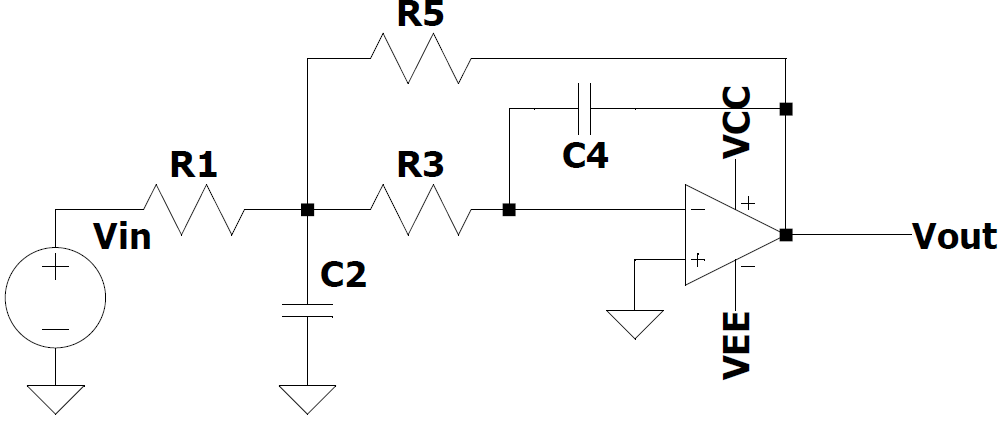
\includegraphics[width=\linewidth]{figuras/MFB.png}
        \centering
        \\ \textbf{(a)}
    \end{minipage}
    \caption{Oi}
    \label{fig:MFB}
\end{figure}

Com base na equação~\ref{eq:H0} e os as proprieades mostradas nas equações~\ref{eq:constante2} e~\ref{eq:inversa}, podemos calcular a sensibilidade de $H_0$ em relação a $R_1$ e $R_5$:	

\begin{equation}
    S^{H_0}_{R_1} = - S^{H_0}_{1/R_1} = -1,
\end{equation}

\begin{equation}
    S^{H_0}_{R_5} = 1.
\end{equation}

Com base na equação~\ref{eq:omega0} e as propriedades mostradas nas equações~\ref{eq:constante2},\ref{eq:inversa} e~\ref{eq:potencia}, podemos calcular a sensibilidade de $\omega_0$ em relação a $R_3$, $R_5$, $C_2$ e $C_4$:

\begin{equation}
    S^{\omega_0}_{R_3} = - S^{\omega_0}_{1/R_3} = -\frac{1}{2} S^{\omega_0}_{R^{-1/2}_3} = -\frac{1}{2},
\end{equation}

\begin{equation}
    S^{\omega_0}_{R_5} = S^{\omega_0}_{C_2} = S^{\omega_0}_{C_4} = S^{\omega_0}_{R_3} = - \frac{1}{2}
\end{equation}

Com base na equação~\ref{eq:Q} e as propriedades mostradas nas equações~\ref{eq:constante2},\ref{eq:inversa} e~\ref{eq:divisao}, podemos calcular a sensibilidade de $Q$ em relação a $R_1$, $R_3$, $R_5$ e $C_2$:

\begin{equation}
    S^{Q}_{x} = S^{\omega_0}_{x} - S^{\omega_0/Q}_{x} \quad \text{(x = $R_1$, $R_3$, $R_5$ e $C_2$)}
\end{equation}

\begin{equation}
    S^{\omega_0/Q}_{C_2} = -S^{\omega_0/Q}_{1/C_2} = -1
\end{equation}

\begin{equation}
    S^{\omega_0/Q}_{R_1} = -S^{\omega_0/Q}_{1/R_1} = -\frac{1/R_1}{1/R_1 + 1/R_3 + 1/R_5}
\end{equation}

\begin{equation}
    S^{\omega_0/Q}_{R_3} = -\frac{1/R_3}{1/R_1 + 1/R_3 + 1/R_5}
\end{equation}

\begin{equation}
    S^{\omega_0/Q}_{R_5} = -\frac{1/R_5}{1/R_1 + 1/R_3 + 1/R_5}
\end{equation}